\section{Results}
\label{sec:results}

\subsection{Real-data benchmark}
\label{sec:experiments-real}

\Cref{tab:method-main-comparison} reports the main real-data comparison.
Classification uses the 21 datasets with results for every method; the full
classification collection has 23 datasets, and \nolinkurl{gisette} and
\nolinkurl{isolet} enter only the comparisons whose methods completed there
(\cref{app:methods} lists the excluded runs). Regression uses all 8
datasets. Within each dataset, scores are first averaged over downstream
learners and the standard $k$ values shared by the compared methods, then
converted to ranks. Lower mean rank is better.

\begin{table}[H]
  \centering
  \footnotesize
  \setlength{\tabcolsep}{5pt}
  \renewcommand{\arraystretch}{0.88}
  \begin{tabular}{@{}l S[table-format=2.2] @{\hspace{2.5em}} l S[table-format=2.2]@{}}
    \toprule
    \multicolumn{2}{c}{Classification} &
    \multicolumn{2}{c}{Regression} \\
    \cmidrule(lr){1-2}\cmidrule(l){3-4}
    \tablehead{Method} & {Mean rank} & \tablehead{Method} & {Mean rank} \\
    \midrule
    RF-RFE & 4.19 & ExtraTrees & 5.00 \\
    XGBoost & 5.81 & CIF & 6.25 \\
    CIF & 5.86 & CatBoost & 6.75 \\
    RF & 5.86 & RF-RFE & 6.88 \\
    LightGBM & 6.05 & RF & 7.63 \\
    Boruta & 6.62 & RT & 8.25 \\
    CatBoost & 6.76 & cforest & 8.75 \\
    ExtraTrees & 7.33 & DT & 9.38 \\
    cforest & 8.33 & Boruta & 9.50 \\
    DT & 8.62 & PC filter & 9.88 \\
    RDC filter & 11.05 & LightGBM & 10.13 \\
    PI & 11.67 & XGBoost & 10.13 \\
    MC filter & 11.86 & RDC filter & 11.00 \\
    RT & 12.81 & CIT & 11.13 \\
    ctree & 12.86 & ctree & 11.38 \\
    CIT & 13.14 & PI & 11.75 \\
    CPI & 14.19 & DC filter & 12.25 \\
    \multicolumn{2}{c}{} & CPI & 15.00 \\
    \bottomrule
  \end{tabular}
  \caption{Main real-data comparison. Ranks are computed within each dataset
  after scores are averaged over downstream learners and the standard $k$ values
  shared by the compared methods, then averaged across datasets. Classification
  uses the 21 datasets with results for every method; regression uses all 8
  datasets. Mean ranks carry no interval here; bootstrap intervals for the
  paired differences and the omnibus tests are in \cref{app:benchmark-stability}.}
  \label{tab:method-main-comparison}
\end{table}

With the selected configurations fixed, CIF ties RF for 3rd of 17
classification methods, 0.05 in mean rank behind XGBoost, and ranks 2nd of 18
regression methods; on the smaller complete-case panels it is tied 6th of 17 and
tied 5th of 18. The regression ordering is descriptive, because the
complete-case Friedman test does not reject at the 0.05 level ($p=0.072$).
\Cref{tab:conditional-inference-comparisons} compares CIF directly with ctree,
cforest, and CIT.
\Cref{app:benchmark-stability} gives the learner-by-$k$ tables
(\cref{tab:classification-learner-k-sensitivity,tab:regression-learner-k-sensitivity}),
pairwise CIF-comparison heatmaps
(\cref{fig:benchmark-pairwise-sensitivity,fig:regression-benchmark-pairwise-sensitivity}),
and seed-sensitivity tables
(\cref{tab:classification-seed-sensitivity,tab:regression-seed-sensitivity});
each analysis reports its dataset count.

\begin{table}[H]
  \centering
  \footnotesize
  \setlength{\tabcolsep}{5pt}
  \renewcommand{\arraystretch}{0.92}
  \begin{tabular}{@{}llS[table-format=2.0]S[table-format=+1.3]S[table-format=+1.3]c@{}}
    \toprule
    \tablehead{Task} & \tablehead{Compared with} & {Datasets} & {Median diff.} & {Mean diff.} & W--L \\
    \midrule
    Classification & ctree & 21 & +0.025 & +0.037 & \winloss{19}{2} \\
    Classification & cforest & 22 & +0.008 & +0.010 & \winloss{17}{5} \\
    Classification & CIT & 23 & +0.022 & +0.032 & \winloss{22}{1} \\
    Regression & ctree & 8 & +0.031 & +0.157 & \winloss{6}{2} \\
    Regression & cforest & 8 & +0.009 & +0.021 & \winloss{6}{2} \\
    Regression & CIT & 8 & +0.015 & +0.234 & \winloss{7}{1} \\
    \bottomrule
  \end{tabular}
  \caption{Direct CIF comparisons against ctree, cforest, and CIT. Differences
  are CIF minus the compared method after averaging within each dataset over
  supported downstream learners and standard values of $k$, summarized over
  datasets by their median and mean; classification uses balanced accuracy and
  regression uses $R^2$, for which the median is the primary summary because
  $R^2$ is unbounded below. W--L reports wins and losses over datasets where
  both methods were run.}
  \label{tab:conditional-inference-comparisons}
\end{table}

\FloatBarrier

\Cref{tab:conditional-inference-comparisons} shows CIF ahead in all six direct
pairings by both the median and the mean over datasets. In regression the
median is the primary summary: $R^2$ is unbounded below, and on the three
\nolinkurl{coepra} datasets (76 to 133 observations, about 5,000 features) the
comparators reach large negative values, so the CIF-minus-ctree and
CIF-minus-CIT means of 0.157 and 0.234 are set by those three datasets while
the medians are 0.031 and 0.015. On the complete-case datasets, CIF is also
ahead of ctree, cforest, and CIT in both tasks. The 95\% bootstrap CIs for the
mean CIF-minus-comparator differences are as follows. Classification (13
datasets): ctree [+0.026, +0.073], cforest [+0.002, +0.024], CIT [+0.027,
+0.062]. Regression (6 datasets): ctree [+0.029, +0.421], cforest [-0.032,
+0.090], CIT [-0.002, +0.766]. The classification intervals and the regression
ctree interval exclude zero; the regression intervals for cforest and CIT cross
it, and all three are wide for the same reason the means are large: six
datasets, three of them with unstable $R^2$.

\paragraph{Mechanism-matched check.}
The CIF margin over cforest mixes the importance mechanism with the way the
trees are grown. Ranked by cforest's own out-of-bag permutation importance
(\cref{sec:experiments-mechanism,tab:cif-perm-check}), CIF leads cforest in
classification by $+0.012$ mean and $+0.006$ median balanced accuracy with 15
wins in 20 datasets, against $+0.011$ for split-ranked CIF, and the two CIF
rankings differ by $+0.001$, so the classification margin does not come from
the importance mechanism. In regression the medians agree, while the means move
with one unstable dataset (\cref{app:cif-perm-check}).

\paragraph{Random forest ranked by out-of-bag permutation importance.}
In the clinical application of \citet{MilletichDownesHirst2026citrees}, an
ordinary random forest loses its high-cardinality preference once it is ranked
by out-of-bag permutation importance rather than by impurity; on the
weak-signal designs of \cref{sec:mechanism} the same ranking keeps it, with a
500-level noise share of 0.47 against 0.38 for impurity at the weakest signal.
\Cref{tab:rf-oobperm-benchmark} adds this permutation-importance forest to the
benchmark: the benchmark's 100-tree random forest is refit on every fold and
ranked by one permutation of each column on each tree's out-of-bag rows, the
mechanism cforest uses, and the ranking is scored exactly as the others. It
ranks 8th of 18 in classification and 6th of 19 in regression, below the
impurity-ranked forest and below CIF on both panels (median differences of
$-0.003$ and $-0.007$ against CIF), and above cforest in classification. With
it present, CIF moves from tied 3rd of 17 to 4th of 18 in classification (mean
rank 6.38, behind RF at 6.19 and XGBoost at 6.24) and stays 2nd in regression.
Ranking the same forest by out-of-bag permutation importance instead of impurity
therefore does not improve its downstream score: the permutation-importance
forest scores below the impurity-ranked one in both tasks.
The permutation step also costs time at high dimension: a median 29 seconds per
fold in classification and 127 in regression against 0.2 seconds for the forest
fit, and 43 and 32 minutes per fold on gisette and dexter, because its work
grows with the number of features times the number of trees. On a
low-dimensional cohort such as the clinical one it is cheap; on the wide
datasets it is not.

\begin{table}[H]
  \centering
  \footnotesize
  \setlength{\tabcolsep}{5pt}
  \begin{tabular}{@{}llrrS[table-format=+1.3]S[table-format=+1.3]c@{}}
    \toprule
    \tablehead{Task} & \tablehead{Compared with} & {Datasets} & {Position} & {Median diff.} & {Mean diff.} & W--L \\
    \midrule
    Classification & CIF & 23 & 8 of 18 & -0.003 & -0.002 & \winloss{11}{12} \\
    Classification & RF & 23 & & -0.004 & -0.004 & \winloss{8}{15} \\
    Classification & cforest & 22 & & +0.005 & +0.009 & \winloss{16}{6} \\
    Regression & CIF & 8 & 6 of 19 & -0.007 & -0.028 & \winloss{3}{5} \\
    Regression & RF & 8 & & -0.002 & -0.032 & \winloss{3}{5} \\
    Regression & cforest & 8 & & +0.002 & -0.007 & \winloss{5}{3} \\
    \bottomrule
  \end{tabular}
  \caption{Random forest ranked by out-of-bag permutation importance as an added
  comparator. Position is its mean-rank position when it joins the all-method
  panels of 21 and 8 datasets (18 classification and 19 regression families);
  differences are the new ranker minus the compared method after averaging
  within each dataset over downstream learners and standard $k$, summarized by
  median and mean over the datasets both completed; balanced accuracy in
  classification, $R^2$ in regression. W--L counts datasets where the new ranker
  is higher or lower. Full ranks and deltas are in
  \texttt{paper\_rf\_oobperm\_method\_aggregate.csv} and
  \texttt{paper\_rf\_oobperm\_pairwise.csv} of the reference release.}
  \label{tab:rf-oobperm-benchmark}
\end{table}

\paragraph{CIF ablations.}
\Cref{tab:cif-ranking-ablation} compares the selected CIF configuration with
four targeted changes on the real-data benchmark datasets: split-count ranking,
disabling bootstrap sampling, disabling feature muting, and using one tree.
Each changed variant is paired with the reference in the same seed and fold.
In classification, reducing CIF to one tree lowers balanced accuracy on every
dataset, by $0.071$ on average, while split-count ranking, disabling bootstrap
sampling, and disabling feature muting change it by at most $0.001$ on average,
with intervals that include zero. Regression is
heterogeneous and the negligible-effect statement does not carry over: the one
tree loses on all eight datasets, by $0.66$ $R^2$ on average and $0.06$ at the
median; split-count ranking and disabling bootstrap sampling lower the mean
$R^2$ by $0.053$ and $0.064$ with intervals that exclude zero, although their
medians are within $0.007$ of zero and the win--loss counts are 2--6 and 4--4;
and disabling feature muting lowers the mean by $0.157$ with a median of zero and
an interval that includes it. The means are pulled down by the three small \nolinkurl{coepra}
datasets, where $R^2$ is unstable across folds: in regression the mean
differences are set by a few datasets while the medians stay near zero, so the
table reports both statistics.

\begin{table}[H]
  \centering
  \footnotesize
  \setlength{\tabcolsep}{4pt}
  \renewcommand{\arraystretch}{1.08}
  \begin{tabular}{@{}llS[table-format=+1.3]S[table-format=+1.3]cc@{}}
    \toprule
    \tablehead{Task} & \tablehead{CIF change} & {Mean diff.} & {Median diff.} & 95\% CI & W--L \\
    \midrule
    Classification & Split-count ranking & -0.001 & 0.000 & [-0.005, +0.002] & 12--9 \\
    Classification & Disable bootstrap & -0.001 & 0.000 & [-0.004, +0.003] & 9--12 \\
    Classification & Disable feature muting & +0.001 & 0.000 & [-0.001, +0.002] & 13--5 \\
    Classification & Use one tree & -0.071 & -0.043 & [-0.101, -0.045] & 0--22 \\
    \addlinespace
    Regression & Split-count ranking & -0.053 & -0.003 & [-0.142, -0.002] & 2--6 \\
    Regression & Disable bootstrap & -0.064 & -0.007 & [-0.128, -0.010] & 4--4 \\
    Regression & Disable feature muting & -0.157 & 0.000 & [-0.468, +0.001] & 4--4 \\
    Regression & Use one tree & -0.658 & -0.059 & [-1.692, -0.054] & 0--8 \\
    \bottomrule
  \end{tabular}
  \caption{CIF ablations on the real-data benchmark. Differences compare each
  changed variant with the selected CIF configuration using split-importance
  ranking, paired within seed and fold. Scores are averaged within each dataset
  over downstream learners, supported standard values of $k$, and the 25 paired
  fold~$\times$~seed replicates. Classification uses balanced accuracy;
  regression uses $R^2$. The confidence intervals are percentile bootstrap
  intervals for the mean over dataset-level differences from 20{,}000
  replicates. Positive values favor the changed CIF variant. W--L counts
  datasets where the changed variant is higher or lower than the reference;
  exact ties are omitted. The classification rows use 22 datasets and the
  regression rows use 8 datasets.}
  \label{tab:cif-ranking-ablation}
\end{table}

\paragraph{RDC projections.}
The RDC rankings are insensitive to the number of random projections. In a
5-seed, 5-fold analysis on four small classification datasets, 20 instead of
10 projections required more than three times the median selector time,
changed mean balanced accuracy by at most 0.0052, and kept at least 95.4
percent mean overlap between the selected feature sets.

The complete-case Friedman tests use dataset-level method means.
Classification: $\chi^2(16)=140.46$, $p<0.001$, Kendall's $W=0.68$.
Regression: $\chi^2(17)=26.15$, $p=0.072$, Kendall's $W=0.26$, which does not
reach the 0.05 level, so the regression rank ordering is a descriptive summary
of the 6-dataset panel rather than evidence of method differences.

The paired bootstrap intervals of CIF against every other method on the same
panels, computed as in \cref{tab:cif-ci-comparisons}, which reports those
against ctree, cforest, and CIT, are unadjusted post-hoc contrasts, 16 in
classification and 17 in regression with no familywise correction, and are
read as descriptive. In classification they exclude zero in CIF's favor against
CIT, ctree, cforest, the single trees, the permutation filters, PI, and CPI;
they exclude zero against CIF for RF-RFE, XGBoost, and LightGBM; and they
include zero for RF, ExtraTrees, CatBoost, and Boruta, so the data do not
resolve the order of CIF among these four. In regression, where the omnibus
test does not reject, no interval excludes zero against CIF, and CIF's
intervals exclude zero only against the filters, PI, CPI, LightGBM, and ctree.
These intervals and rank summaries describe the
benchmark-selected configurations. The LODO analysis below checks whether those
configurations are stable under one-dataset holdout.

The complete-case panels rank CIF lower than the main table does, and the
LODO reselection accounts for little of the difference. On the 13-dataset
classification panel, the benchmark-selected CIF configuration has mean rank
6.38 (tied 6th of 17); LODO reselection moves it to 6.85 (8th) and reselects the
main-benchmark configuration in 11 of 13 holdouts. On the 6-dataset regression
panel, the fixed configuration has mean rank 7.00 (tied 5th of 18) and LODO
moves it to 7.33 (6th), behind ExtraTrees, CatBoost, RF-RFE, RF, and RT,
reselecting the global configuration in 4 of 6 holdouts. The 3rd and 2nd
places in \cref{tab:method-main-comparison} are therefore properties of the
21- and 8-dataset panels: the smaller complete-case panels move CIF from tied
3rd to tied 6th in classification and from 2nd to tied 5th in regression, and
configuration reselection adds less than half a rank.

On the 21- and 8-dataset panels themselves, reselection moves CIF from 5.86 (tied 3rd) to 6.10 (5th) in classification and from 6.25 to 6.50 (2nd in both) in regression, reselecting the benchmark configuration in 20 of 21 and 7 of 8 holdouts, with held-out scores lower by 0.002 balanced accuracy and 0.008 $R^2$ (\cref{tab:lodo-config-sensitivity-allmethod}). Every single-configuration family keeps its score, and its rank moves only through the reselection of others, by at most 0.05 in classification and 0.125 (one place on eight datasets) in regression.
\Cref{tab:cif-ci-comparisons,tab:lodo-config-sensitivity}
give the confidence intervals and LODO details.

\Cref{tab:cif-breadth-summary} reports how often CIF appears in the top half or
top 3 and how often it beats tree baselines.

\begin{table}[H]
  \centering
  \footnotesize
  \setlength{\tabcolsep}{6pt}
  \renewcommand{\arraystretch}{1.0}
  \begin{tabular}{@{}lcc@{}}
    \toprule
    \tablehead{Summary} & Classification & Regression \\
    \midrule
    Main rank & \countfrac{3.5}{17} & \countfrac{2}{18} \\
    Top half & \countfrac{17}{21} & \countfrac{5}{8} \\
    Top 3 & \countfrac{4}{21} & \countfrac{2}{8} \\
    Win vs ctree & \countfrac{19}{21} & \countfrac{6}{8} \\
    Win vs cforest & \countfrac{17}{22} & \countfrac{6}{8} \\
    Win vs CIT & \countfrac{22}{23} & \countfrac{7}{8} \\
    Win vs DT & \countfrac{16}{23} & \countfrac{5}{8} \\
    Win vs RT & \countfrac{21}{23} & \countfrac{5}{8} \\
    \bottomrule
  \end{tabular}
  \caption{Dataset breadth for the selected CIF configuration. Top half and
  Top 3 counts use the datasets from \cref{tab:method-main-comparison}. Direct
  win rows use datasets where both methods were run. The fractional
  classification main rank reflects a tie with RF. Counts carry no interval; paired intervals for CIF against ctree, cforest, and CIT on the complete-case panels are in \cref{tab:cif-ci-comparisons}.}
  \label{tab:cif-breadth-summary}
\end{table}

CIF's position rests on breadth rather than on a few strong datasets: it is in
the top half on 17 of 21 classification and 5 of 8 regression datasets but in
the top 3 on only 4 of 21 and 2 of 8, and it beats DT on 16 of 23 and RT on 21
of 23 classification datasets, while in regression both single-tree comparisons
are close (5 of 8 each, with a mean difference near zero against RT).

\Cref{fig:k-trajectory,fig:regression-k-trajectory} report mean rank separately
by $k$. Because the dataset count falls as $k$ grows, the trend is read on the
constant complete-case panels of 13 classification and 6 regression datasets:
in classification CIF improves with $k$, from 7th and 8th of 17 at $k \le 10$
to 4th at $k=100$ (mean ranks 7.8, 7.7, 6.5, 6.2, and 5.7), and in regression
its position varies between 3rd and 7th of 18 with no monotone trend in $k$
(mean ranks 8.2, 8.3, 6.3, 7.0, and 7.0).

\FloatBarrier

\begin{figure}[H]
  \centering
  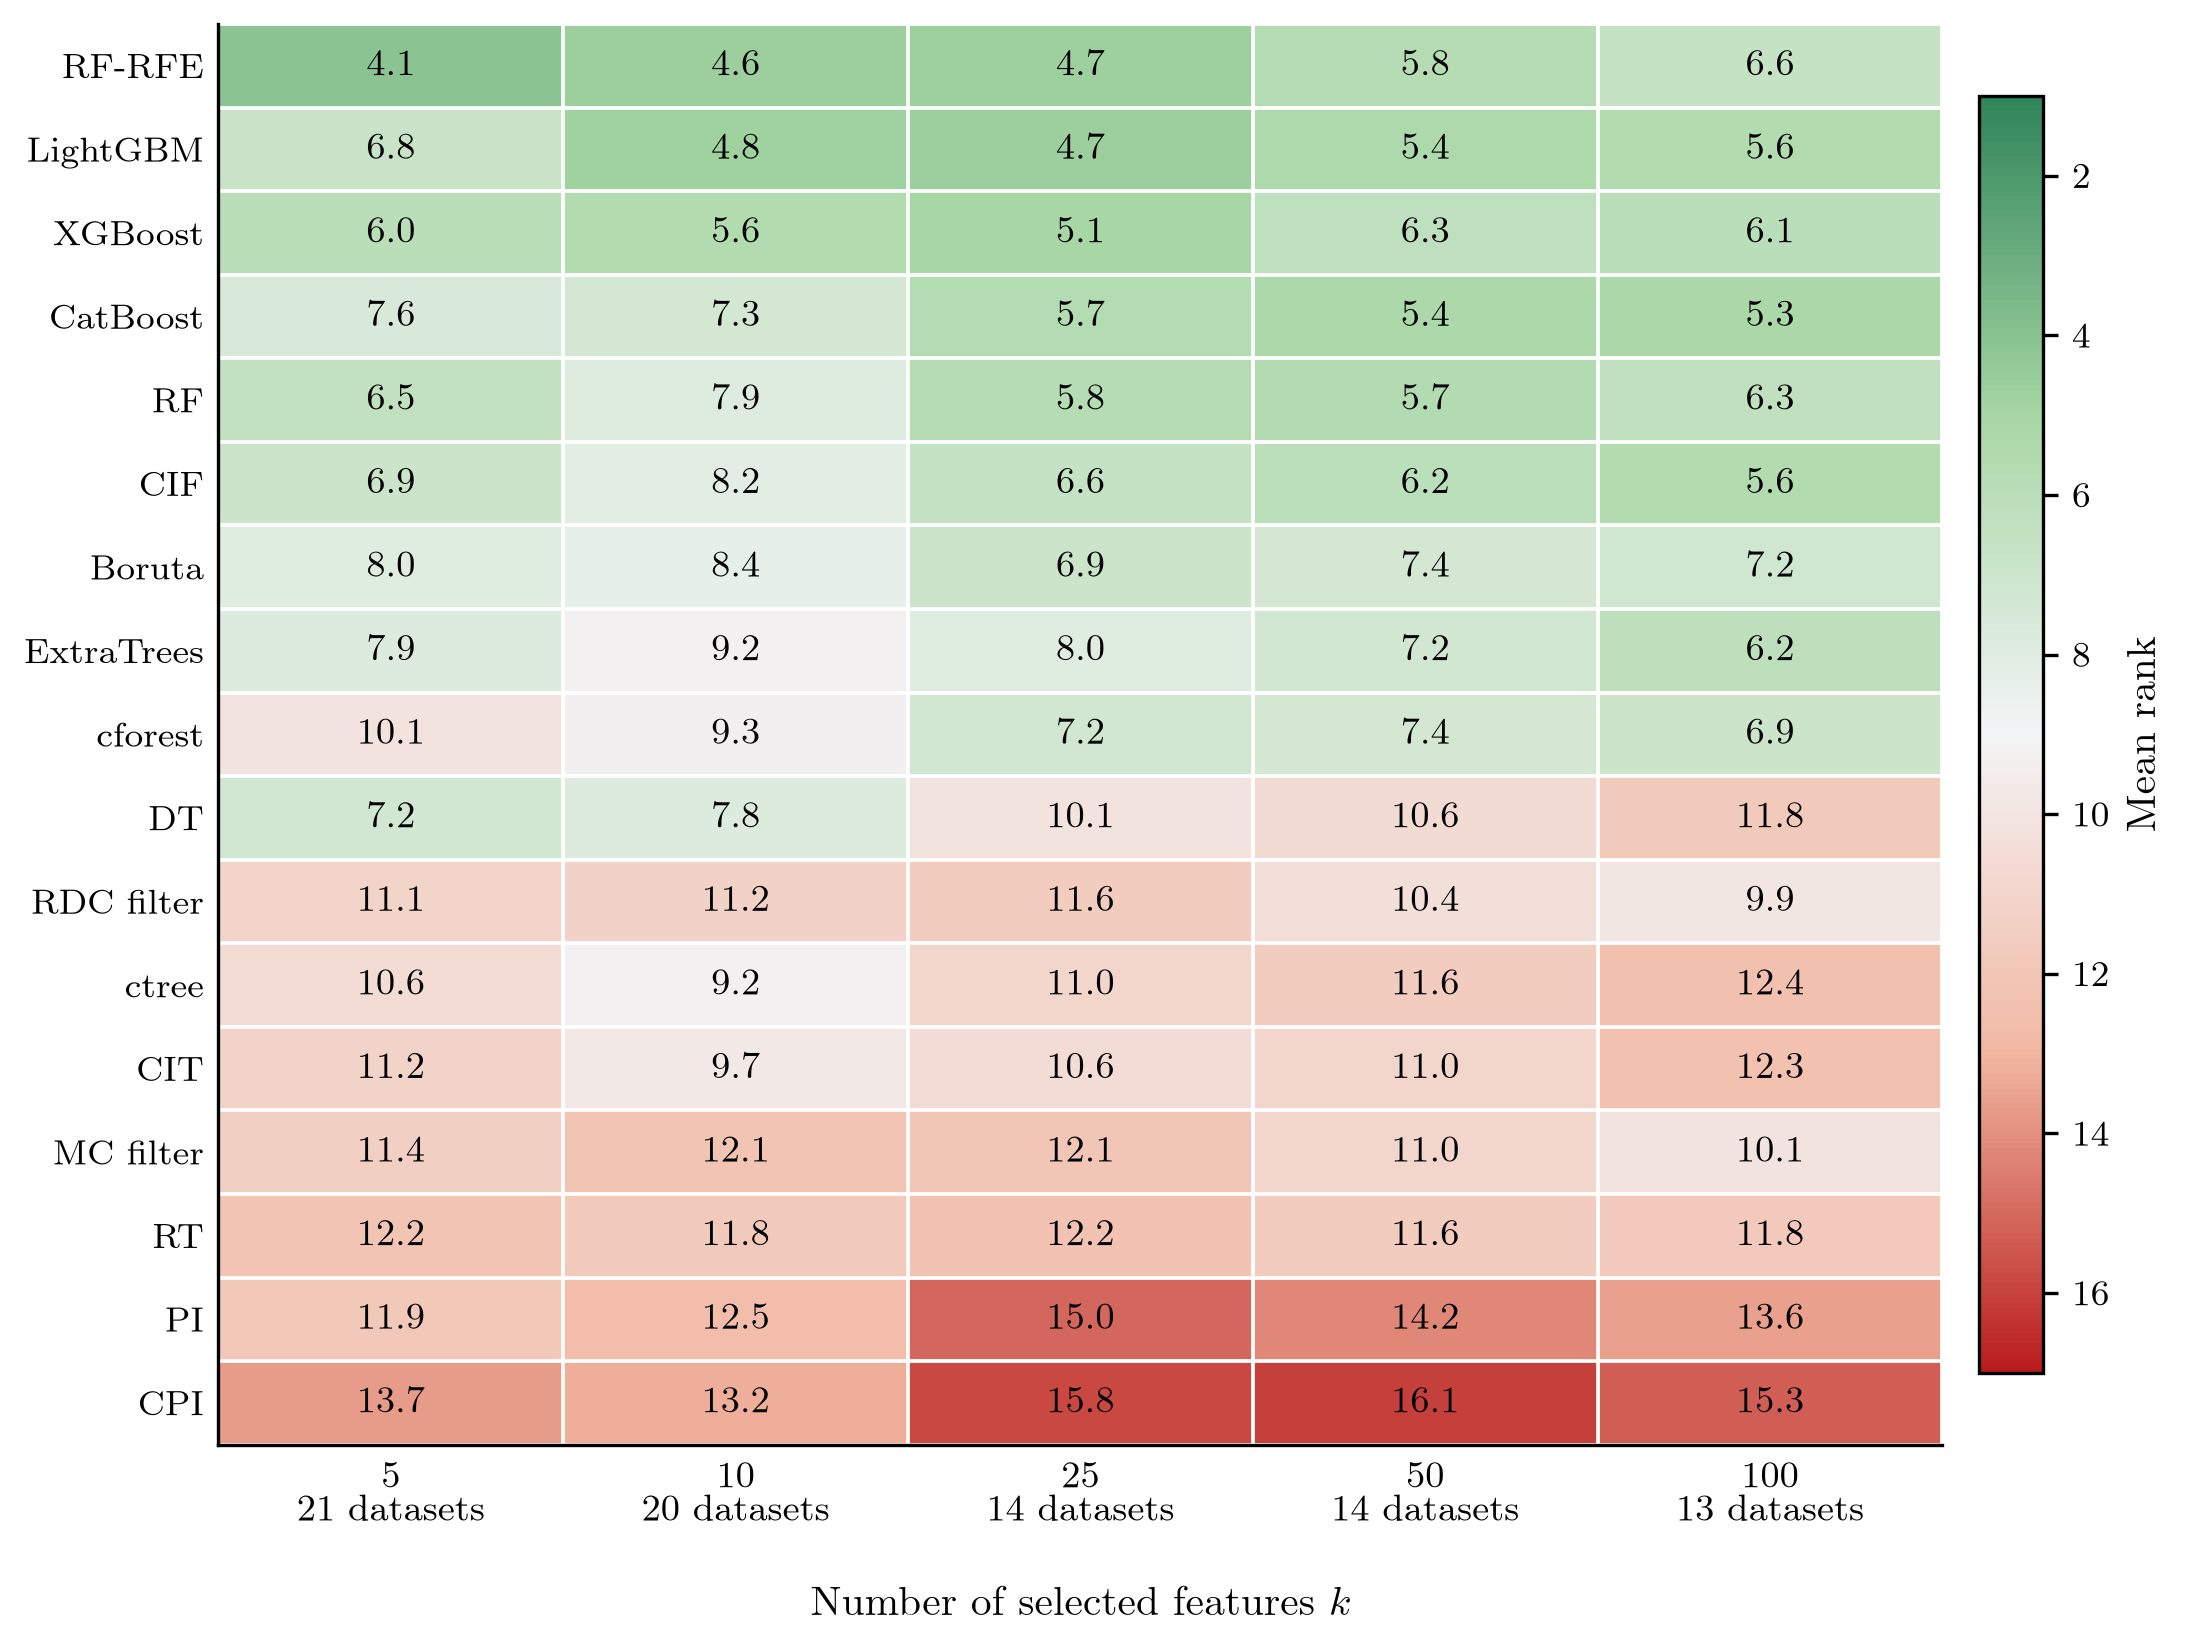
\includegraphics[width=0.86\linewidth]{figures/classification_k_trajectory.png}
  \caption{Classification mean rank by number of selected features. Rows show
  all 17 feature selection methods in the classification benchmark, averaged
  across downstream models at each value of $k$. Lower ranks are better.
  The columns for $k=5,10,25,50,100$ use 21, 20, 14, 14, and 13 datasets,
  respectively. Each cell is a mean over the datasets in that column with no interval; the seed and learner sensitivity tables in \cref{app:benchmark-stability} bound its variation.}
  \label{fig:k-trajectory}
\end{figure}

\begin{figure}[H]
  \centering
  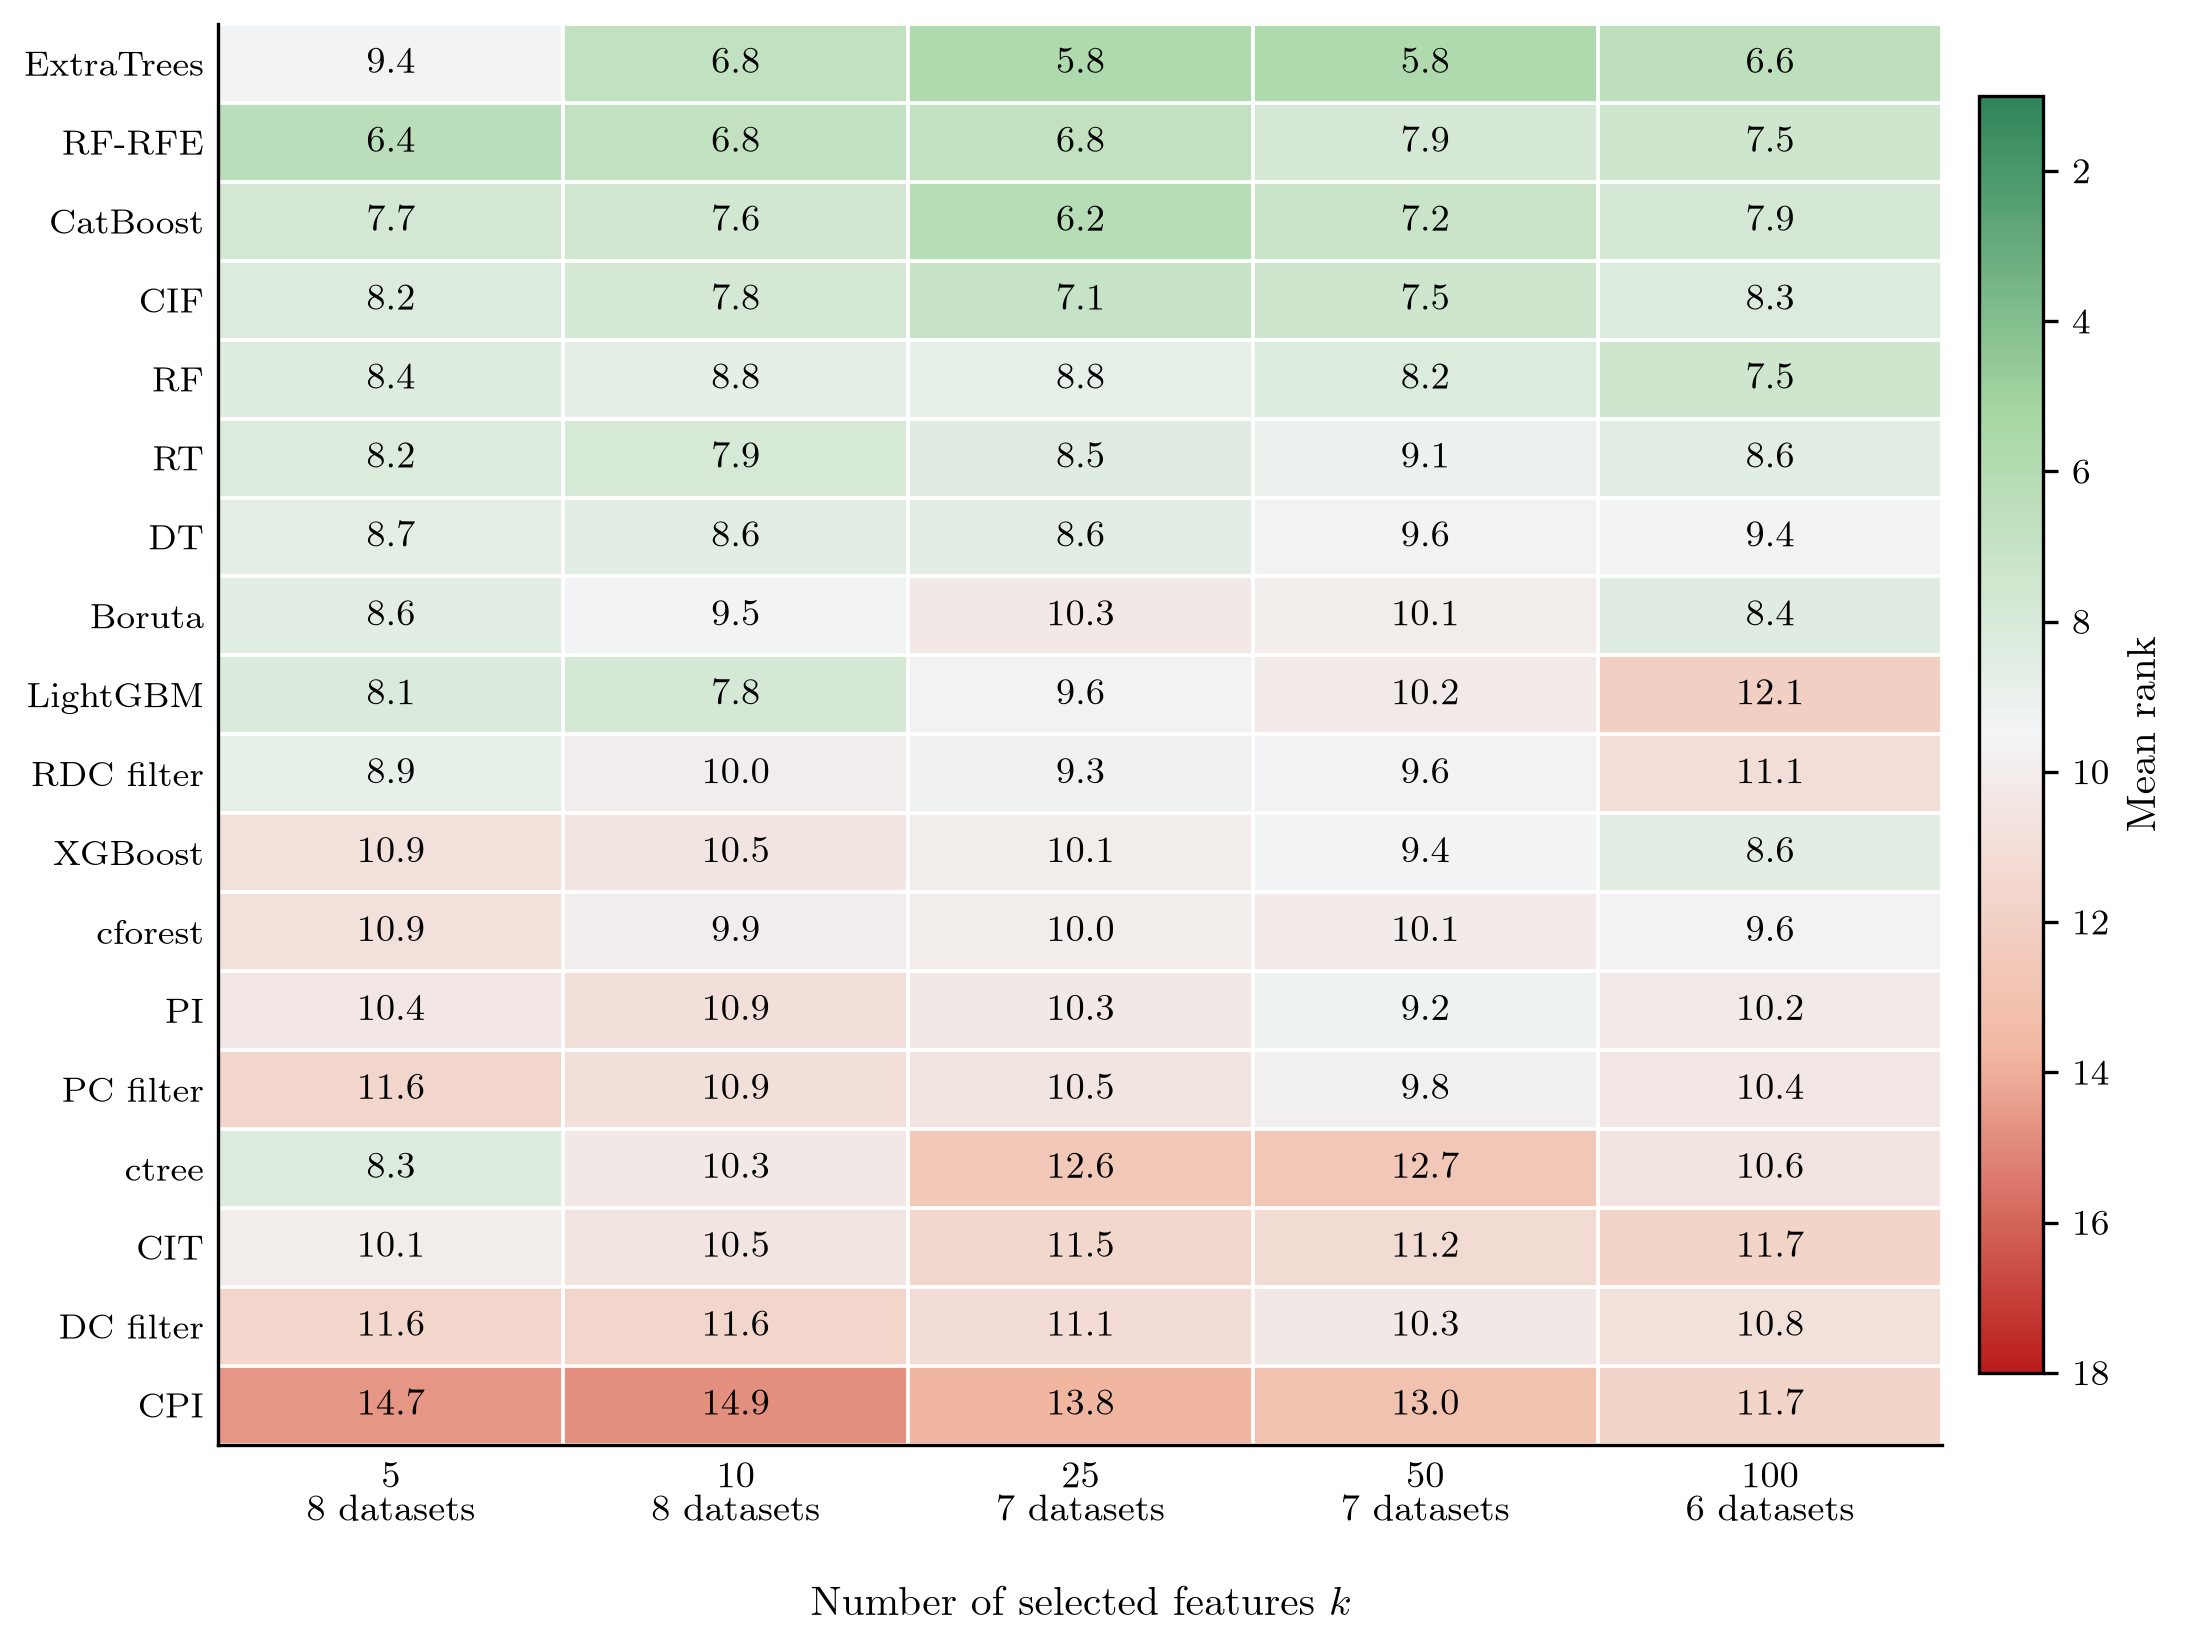
\includegraphics[width=0.86\linewidth]{figures/regression_k_trajectory.png}
  \caption{Regression mean rank by number of selected features. Rows show all
  18 feature selection methods in the regression benchmark, averaged across
  downstream models at each value of $k$. Lower ranks are better. The columns
  for $k=5,10,25,50,100$ use 8, 8, 7, 7, and 6 datasets, respectively. Each cell is a mean over the datasets in that column with no interval; the seed and learner sensitivity tables in \cref{app:benchmark-stability} bound its variation.}
  \label{fig:regression-k-trajectory}
\end{figure}

\FloatBarrier

\subsection{Runtime ablations}
\label{sec:results-practical}

The runtime ablations identify which benchmark settings have the largest effect
on fitting time and report how much the ranking scores move when those settings
change. Each row switches one control off and reports elapsed wall-clock fit time
relative to the selected configuration for the same estimator, as the median
over datasets of the per-dataset ratio, in each of the four task groups
(classification and regression, real and synthetic). Ratios above 1 are slower
than the reference and ratios below 1 are faster. Scanning and early stopping are
independent switches, so each row measures one mechanism. CIT and CIF are shown
separately because the CIT run records fit time and synthetic top-10 feature
recovery, while the CIF runs also record downstream score changes.
\Cref{app:complexity-details} links each ablation to the affected work terms.

\begin{table}[H]
  \centering
  \footnotesize
  \setlength{\tabcolsep}{6pt}
  \begin{tabular}{@{}lcc@{}}
    \toprule
    \tablehead{CIT change} & Runtime ratio & \shortstack{Largest top-10\\F1 change} \\
    \midrule
    Disable adaptive stopping (minimum budget) & 0.88--0.99$\times$ & 0 \\
    Auto budget, adaptive stopping & 1.18--1.56$\times$ & $\le 0.016$ \\
    Auto budget, no early stopping & 3.8--8.2$\times$ & $\le 0.016$ \\
    Disable threshold scanning & 2.7--34$\times$ & $\le 0.033$ \\
    Disable feature scanning & 0.81--3.0$\times$ & $\le 0.058$ \\
    Exact threshold search & 0.91--1.10$\times$ & $\le 0.004$ \\
    Disable feature muting & 0.97--0.98$\times$ & 0 \\
    Remove feature and threshold corrections & 0.52--1.8$\times$ & $\le 0.063$ \\
    \bottomrule
  \end{tabular}
  \caption{CIT runtime ablations. Runtime ratios are medians over datasets of the
  per-dataset ratio to the selected CIT configuration, given as the range over the
  four task groups; five seeds per dataset on 23 datasets (15 classification and 8
  regression; 9 real and 14 synthetic). The F1 column is the largest change in mean top-10 F1 on
  the synthetic datasets across the task groups. Fits ran on one 32-core
  machine with the full thread pool per tree; every time is the second of two
  identical fits, so compilation is excluded. The two auto-budget rows use the
  auto budget, which exceeds the $\lceil 1/\alpha \rceil$ floor, so the
  stopping rule can act.}
  \label{tab:cit-runtime-hyperparams}
\end{table}

\paragraph{CIT runtime ablations.}
\Cref{tab:cit-runtime-hyperparams} separates the permutation budget from the
stopping rule. At the benchmark's minimum budget, adaptive stopping is inert by
construction (\cref{prop:adaptive-size}): the budget equals the floor below
which the rule cannot stop, so switching it off changes fitting time by
0.88--0.99$\times$ and leaves every tree, and therefore every recovery score,
unchanged. Where the rule can act it earns its place: at the auto budget the
adaptive tree costs 1.18--1.56$\times$ the selected configuration at the
minimum budget, while the same budget with no stopping costs 3.8--8.2$\times$,
so within each task group adaptive stopping brings the larger budget's tree to
0.14--0.37 of its no-stopping time at a recovery change of at most 0.016.

The control that matters for a single tree is the threshold scan: testing
candidate thresholds in order of promise and stopping at the first rejection
makes fits 2.7--34$\times$ faster than testing every candidate, with the
largest ratio on the real regression datasets, where predictors admit the full
257 candidates. Feature scanning matters less for a single tree
(0.81--3.0$\times$, faster in one group because the prescan itself has a
cost), and exact threshold search and feature muting are within a few percent
of the selected configuration. Removing the feature and threshold corrections
changes the statistical rule: trees grow from a mean depth of 6.5 and 7.2 to
10.7 and 13.4 levels and top-10 recovery moves by up to 0.063, so the
corrections are not a runtime control.

The pattern holds on the 14 Benchmark-size datasets (up to 20,000 observations
and 5,000 features; five seeds each): switching adaptive stopping off changes
single-tree time by 0.80--1.01$\times$ (medians 0.97 in classification and
0.88 in regression), threshold scanning saves a median 17$\times$ in
classification and up to 45$\times$ on spam, and removing the two corrections
runs in 0.01--1.26$\times$ the time of the selected configuration. The largest
single-tree time is gisette at 29 minutes, where the feature correction over
5,000 features sets a large minimum budget for each feature test.

\begin{table}[H]
  \centering
  \footnotesize
  \setlength{\tabcolsep}{6pt}
  \begin{tabular}{@{}lccc@{}}
    \toprule
    \tablehead{CIF change} & Runtime ratio & \shortstack{Downstream\\score change} & \shortstack{Synthetic feature\\recovery change} \\
    \midrule
    Disable adaptive stopping & 0.96--1.00$\times$ & 0 & 0 \\
    Auto budget, adaptive stopping & 1.30--2.0$\times$ & -- & $\le 0.030$ \\
    Auto budget, no early stopping & 5.8--15$\times$ & -- & $\le 0.025$ \\
    Disable threshold scanning & 7.9--30$\times$ & $\le 0.003$ & $\le 0.010$ \\
    Disable feature scanning & 1.0--5.2$\times$ & $\le 0.003$ & $\le 0.008$ \\
    Exact threshold search & 1.3--19$\times$ & $\le 0.009$ & $\le 0.018$ \\
    Histogram with 32 bins & 0.05--0.14$\times$ & $\le 0.008$ & $\le 0.013$ \\
    Disable feature muting & 0.91--1.00$\times$ & $\le 0.001$ & $\le 0.003$ \\
    Disable bootstrap sampling & 0.94--1.69$\times$ & $\le 0.012$ & $\le 0.011$ \\
    Max-type Stage~B test & 0.14--0.61$\times$ & $\le 0.005$ & $\le 0.007$ \\
    Remove feature and threshold corrections & 0.03--0.34$\times$ & $\le 0.004$ & $\le 0.011$ \\
    \bottomrule
  \end{tabular}
  \caption{CIF runtime ablations with score changes. Runtime ratios are medians
  over datasets of the per-dataset ratio to the selected CIF configuration,
  given as the range over the four task groups; five seeds per dataset on 23
  datasets. The exact-threshold and 32-bin rows come from the threshold-search
  ablation and compare with the 256-bin histogram reference. The score columns
  give the largest absolute change in the dataset-mean downstream score and in
  synthetic feature recovery across the task groups; inequality entries are
  rounded upward to the nearest 0.001. The auto-budget rows come from the CIT/CIF
  runtime ablation, which records synthetic recovery but no downstream score.
  Forests fit 100 trees with one worker per tree and one Numba thread per worker
  on a 32-core machine; every time is the second of two identical fits.}
  \label{tab:cif-runtime-hyperparams}
\end{table}

\paragraph{CIF runtime ablations.}
\Cref{tab:cif-runtime-hyperparams} shows the same pattern for forests.
Adaptive stopping is inert at the minimum budget (0.96--1.00$\times$, no score
change). The result does not depend on how trees are scheduled: a forest with
one worker and the full thread pool inside each tree changes fitting time by
0.95--1.01$\times$ when the rule is switched off, on the 21 runtime datasets
other than waveform and california. Where the rule can act, at the auto budget,
the adaptive forest costs 1.30--2.0$\times$ the selected configuration at the
minimum budget and the same budget with no stopping 5.8--15$\times$, so the
adaptive forest runs in 0.11--0.25 of its no-stopping time within each task
group, with synthetic recovery changes of at most 0.030.

The threshold scan is again the dominant control, at 7.9--30$\times$ by group
medians, and the number of candidates is the next: exact threshold search is
1.3--19$\times$ slower than the 256-bin histogram and a 32-bin histogram is
7--21$\times$ faster, with downstream score changes of at most 0.009 and
recovery changes of at most 0.018. Feature scanning costs 1.0--5.2$\times$,
with its largest effect on the real regression datasets. The max-type rule fits
in 0.14--0.61 of the selected configuration's time with downstream changes of
at most 0.005; \cref{sec:results-stageB} reports its calibration, power, and
ranking effect. Removing the feature and threshold corrections gives the
largest speedup for CIF, and is faster for CIT in three of the four groups, but
it changes the statistical rule and yields deeper trees with more selected
features, so the selected configuration keeps both corrections. On the 14
Benchmark-size datasets the forest's adaptive-stopping ratio is
0.99--1.34$\times$ (medians 1.00 and 1.03).
\FloatBarrier

\subsection{Stage~B construction comparison}
\label{sec:results-stageB}

Both Stage~B rules control the false-split rate. At matched realized size the
max-type rule is about 0.006 less powerful, with per-cell differences within
the Monte Carlo error of the design (\cref{tab:stageB-only}), while at a common
nominal level it splits more often because its size is closer to that level
(\cref{tab:stageB-power}); it is also cheaper on continuous predictors and
slightly less precise in where it places the threshold.

The complete-node false-split rate is below 0.05 for both rules in all 36
design cells, 72 measurements pooled over five seeds
(\cref{tab:stageB-calibration}); the rules differ in how far below. Under the
per-threshold rule the rate falls as the bin setting grows, from 0.0196 at 16
bins to 0.0070 at 256 in classification with $n=500$ and no stopping, because
adjacent thresholds induce nearly identical splits and the union bound charges
for each. Under the max-type rule it stays between 0.028 and 0.038 in every cell
and rises slightly with the bin setting, with cell means of 0.032, 0.034, and
0.034. These complete-node rates are dominated by the Stage~A feature test,
which must first reject over five independent predictors, so they bound the
Stage~B threshold test from below rather than measure it.

The Stage-B-only study (\cref{tab:stageB-only}), which fixes the tested
predictor without the response and disables the Stage~A feature test, measures
the threshold test itself. At nominal level 0.05 the per-threshold rule has
size 0.000--0.027, with means of 0.018, 0.011, and 0.006 at 16, 64, and 256
bins, and the max-type rule 0.023--0.044, with means of 0.033, 0.035, and
0.035; every 95\% Clopper--Pearson upper limit is below 0.056, and the cells
whose intervals include 0.05 are max-type cells at 64 and 256 bins. Both rules
are therefore valid at a fixed node for a predictor fixed without the response,
and the reverse cardinality bias of \cref{sec:method} appears as the
per-threshold size falling by a factor of three across the bin settings while
the max-type size does not move.

\begin{table}[H]
  \centering
  \footnotesize
  \setlength{\tabcolsep}{5pt}
  \begin{tabular}{@{}lrrrrrr@{}}
    \toprule
     & & & \multicolumn{2}{c}{Per-threshold} & \multicolumn{2}{c}{Max-type} \\
    \tablehead{Task} & $n$ & Bins & Adaptive & No stopping & Adaptive & No stopping \\
    \midrule
    Classification & 100 & 16 & 0.0182 & 0.0183 & 0.0342 & 0.0352 \\
     & 100 & 64 & 0.0127 & 0.0130 & 0.0353 & 0.0370 \\
     & 100 & 256 & 0.0091 & 0.0096 & 0.0360 & 0.0384 \\
     & 200 & 16 & 0.0200 & 0.0203 & 0.0326 & 0.0342 \\
     & 200 & 64 & 0.0144 & 0.0147 & 0.0333 & 0.0344 \\
     & 200 & 256 & 0.0086 & 0.0092 & 0.0329 & 0.0345 \\
     & 500 & 16 & 0.0196 & 0.0196 & 0.0295 & 0.0314 \\
     & 500 & 64 & 0.0142 & 0.0142 & 0.0322 & 0.0332 \\
     & 500 & 256 & 0.0072 & 0.0070 & 0.0319 & 0.0339 \\
    Regression & 100 & 16 & 0.0272 & 0.0269 & 0.0315 & 0.0328 \\
     & 100 & 64 & 0.0174 & 0.0185 & 0.0337 & 0.0348 \\
     & 100 & 256 & 0.0138 & 0.0145 & 0.0335 & 0.0347 \\
     & 200 & 16 & 0.0282 & 0.0287 & 0.0323 & 0.0347 \\
     & 200 & 64 & 0.0234 & 0.0237 & 0.0351 & 0.0368 \\
     & 200 & 256 & 0.0124 & 0.0127 & 0.0356 & 0.0380 \\
     & 500 & 16 & 0.0262 & 0.0264 & 0.0286 & 0.0295 \\
     & 500 & 64 & 0.0198 & 0.0202 & 0.0288 & 0.0311 \\
     & 500 & 256 & 0.0106 & 0.0108 & 0.0285 & 0.0315 \\
    \bottomrule
  \end{tabular}
  \caption{False-split rate of a depth-one tree under the global null at level
  0.05, by Stage~B rule and stopping mode, over 10,000 replicates per
  cell (five seeds of 2,000) with five independent Gaussian predictors and an independent response. Bins is the histogram threshold setting; the realized candidate count is one more than the setting, capped at the number of distinct values. Every 95\% Clopper--Pearson interval lies below 0.05 (largest upper limit 0.042); the widest half-width is below 0.004.}
  \label{tab:stageB-calibration}
\end{table}

The cost difference is where the rules separate (\cref{tab:stageB-scaling},
\cref{app:stageB-tables}; all three arms timed in one run). With no stopping,
one tree at the 256-bin setting takes 3.5 seconds at $n=1{,}000$, 14 seconds at
$n=4{,}000$, and 59 seconds at $n=16{,}000$ under the per-threshold rule in
classification (0.8, 8.8, and 54 seconds in regression); the max-type rule
takes 0.3, 1.4, and 6.3 seconds at the same settings. The ratio grows with the
bin setting as the $K^2/\alpha$ against $BK$ accounting predicts: at 16 bins
the max-type rule is 1.1--1.3 times slower, because its 999 permutations exceed
the 340 the per-threshold rule needs for 17 candidates, while the no-stopping
ratio is 1.5--2.1 at 64 bins and 2.8--13 at 256. Adaptive stopping shortens the
per-threshold test once its budget exceeds the $\lceil 1/\alpha \rceil$
floor, by 1.2--1.6$\times$ at 16 bins, 2.2--3.2$\times$ at 64, and
3.8--7.8$\times$ at 256, so with adaptive stopping the max-type advantage is
1.0--1.3 at 16 bins, 1.4--2.1 at 64, and 2.2--7.7 at 256.

The fixed-budget control arm shows why the per-threshold rule needs its scaled
budget. Held at 999 permutations per candidate, the rule still splits at 16
bins and is faster than the scaled rule (0.55 and 0.65 seconds against 0.75
and 0.82 at $n=16{,}000$). At 64 and 256 bins it is cheaper still (0.84 to
0.89 and 3.3 to 3.5 seconds at $n=16{,}000$, against 3.3 to 3.6 and 55 to 59
for the scaled rule and 2.1 to 2.2 and 6.3 for the max-type rule), but it never splits
(size 0, power 0, depth 0 in every cell; \cref{tab:stageB-fixed-budget}),
because $\alpha/K$ falls below the resolution $1/(B+1)$. The $K^2/\alpha$
budget is therefore what the per-threshold rule needs in order to reject, and
the max-type rule is the construction that resolves the level at $999K$
permutation statistics.

Depth barely separates the rules on these data: over the grid the max-type
trees have 5.0--10.7 levels and the per-threshold trees 4.0--10.0 under either
stopping mode. The planted signal is linear in three of the ten predictors, so
depth reflects both power at small nodes and splits on noise; the real-data
scores are the measure of which trees predict better.

On the six Stage~B real datasets (\cref{tab:stageB-real},
\cref{app:stageB-tables}), with scores taken as the median over five seeds of
the fold assignment, the max-type rule exceeded the per-threshold rule in 8 of
the 12 dataset and stopping-mode cells and equalled it in one: by 0.016 and
0.026 balanced accuracy on vowel, 0.049 and 0.026 $R^2$ on facebook, 0.060 and
0.033 on imports-85, and 0.008 and 0.005 on residential; on page-blocks it was
lower by 0.018 and 0.020, and on spam lower by 0.006 with adaptive stopping and
equal with no stopping. Its fitting time was 1.2 to 2.4 times shorter with
adaptive stopping and 1.0 to 8.3 times shorter with no stopping on the four
datasets whose predictors admit many candidates per node, with the largest
savings on page-blocks and facebook. It was slower on residential, by 16
percent with adaptive stopping and 10 percent with no stopping, and equal on
imports-85, whose nodes admit few candidates. The fitted depths agree within
about one level (per-threshold 5.4--11.4, max-type 4.8--12.4). The Spearman
agreement of the two rules' feature importances ranges from 0.36 to 0.88, so
the max-type rule produces a different ranking rather than a faster route to
the same one.

In the head-to-head forest timing (\cref{sec:experiments-h2h}), the max-type
rule is 10--27$\times$ faster than the per-threshold rule on the synthetic
Gaussian cells at $n\le 8{,}000$ and 21--36$\times$ faster at $n=32{,}000$
(13--36$\times$ on the $p\in\{20,100\}$ cells that
\citet{MilletichDownesHirst2026citrees} tabulate). The smaller ratios on the
mixed runtime panel of \cref{tab:cif-runtime-hyperparams}, 1.6--7$\times$,
arise where nodes admit few candidates. On the ten real datasets it reduces
madelon from 21 to 2.6 seconds, gamma from 44 to 21 seconds, and isolet from 18
to 9.1 seconds, and changes the other seven by at most 1.6 seconds.

The power study plants a step in one of five Gaussian predictors and records
how often a depth-one tree splits at all and how often on the planted
predictor; \cref{tab:stageB-power} (\cref{app:stageB-tables}) reports the
split rate at a common nominal level, and \cref{tab:stageB-only} the comparison
at matched size. At a common nominal level of 0.05 the max-type rule splits
more often than the per-threshold rule in every cell short of saturation, by
0.03 on average and up to 0.12 in the complete-node design and by 0.10 on
average in the Stage-B-only study. The gap grows with the candidate count, from
0.015 at 16 bins to 0.029 at 64 and 0.049 at 256 in the complete-node design,
because the max-type power is flat in the bin setting while the per-threshold
power falls as the threshold correction tightens. That nominal-level gap is a
size gap, not a power gap.

Matching the two rules at the same realized size in the Stage-B-only study
(\cref{tab:stageB-only}) removes it: the max-type minus per-threshold
difference in size-matched power ranges from $-0.054$ to $+0.034$ over the 108
cell and effect combinations, with mean $-0.006$ and no trend in the bin
setting ($-0.005$, $-0.008$, and $-0.006$ at 16, 64, and 256 bins). In four of
the nine classification cells (64 bins at $n=100$ and 256 bins at every $n$)
and one regression cell ($n=500$, 256 bins) the per-threshold rule does not
reach realized size 0.05 within the nominal grid, its size at nominal 0.50
being 0.031--0.046, so the match in those cells is at that largest realized
size; the other 13 cells match at 0.05. Adaptive stopping and no stopping agree
within 0.014 in every cell.

The two reruns of \cref{sec:experiments-stageB}, whose results are in
\texttt{paper\_stageb\_power\_\allowbreak replicates.csv} of the reference
release, bound the Monte Carlo error of that comparison. With the larger
replicate counts of the fourth seed, the size-matched difference is $-0.006$
on average across the 96 cell and effect combinations completed (range
$-0.040$ to $+0.018$); the 12 combinations of the 256-bin cells at $n=500$, the
$K^2/\alpha$ worst case, were not completed at this replicate count. A
parametric bootstrap of the whole matching procedure, resampling every null and
alternative count and redoing the interpolation, puts a standard error of
about 0.017 on each difference, so the smallest difference the design could
detect is about 0.03, and one of the 96 exceeds two standard errors.

With the off-centre step, the difference is $-0.004$ on average (range
$-0.051$ to $+0.039$, bootstrap standard error about 0.038, detectable
difference about 0.08), and none of the 108 exceeds two standard errors. The
Stage-B-only sizes at nominal 0.05 stay at 0.000--0.026 for the per-threshold
rule and 0.018--0.046 for the max-type rule.

The cost of the joint test is precision, measured on each rule's own
detections, which are not the same replicates. The max-type threshold sits a
median 0.19 standard deviations from the planted cut, against 0.15 for the
per-threshold rule, and 87 rather than 90 percent of its detections fall on the
planted predictor.

Pooled over cells, the size-matched power loss is small and consistent: the
max-type rule is lower in 67 of the 108 cell and effect combinations and higher
in 25. The mean difference is $-0.006$, with a 95 percent bootstrap interval of
$-0.011$ to $-0.002$ that resamples the 18 cells, keeping the effects and
stopping modes of a cell together, and $-0.005$ ($-0.009$ to $-0.002$) over the
13 cells matched at size 0.05. The fourth-seed and off-centre reruns give
$-0.006$ ($-0.008$ to $-0.003$) and $-0.004$ ($-0.008$ to $0.000$), the second
interval reaching zero. What the max-type rule gains at a fixed nominal level
is the size that the threshold correction gives up.

\begin{table}[H]
  \centering
  \footnotesize
  \setlength{\tabcolsep}{4pt}
  \begin{tabular}{@{}lrrrrrrrrr@{}}
    \toprule
     & & & \multicolumn{4}{c}{Size at nominal 0.05} & & \multicolumn{2}{c}{Size-matched power} \\
     & & & \multicolumn{2}{c}{Per-threshold} & \multicolumn{2}{c}{Max-type} & Match & & \\
    \tablehead{Task} & $n$ & Bins & Adapt. & None & Adapt. & None & size & Per-thr. & Max-type \\
    \midrule
    Classification & 100 & 16 & 0.013 & 0.013 & 0.032 & 0.033 & 0.050 & 0.390 & 0.379 \\
     & 100 & 64 & 0.007 & 0.007 & 0.036 & 0.039 & 0.044 & 0.385 & 0.354 \\
     & 100 & 256 & 0.007 & 0.007 & 0.036 & 0.042 & 0.034 & 0.335 & 0.318 \\
     & 200 & 16 & 0.010 & 0.011 & 0.037 & 0.039 & 0.050 & 0.643 & 0.618 \\
     & 200 & 64 & 0.008 & 0.009 & 0.035 & 0.039 & 0.050 & 0.630 & 0.615 \\
     & 200 & 256 & 0.003 & 0.003 & 0.039 & 0.039 & 0.031 & 0.562 & 0.538 \\
     & 500 & 16 & 0.015 & 0.015 & 0.032 & 0.037 & 0.050 & 0.958 & 0.953 \\
     & 500 & 64 & 0.007 & 0.007 & 0.029 & 0.035 & 0.050 & 0.961 & 0.964 \\
     & 500 & 256 & 0.000 & 0.001 & 0.023 & 0.032 & 0.034 & 0.958 & 0.952 \\
    Regression & 100 & 16 & 0.019 & 0.019 & 0.023 & 0.031 & 0.050 & 0.292 & 0.281 \\
     & 100 & 64 & 0.013 & 0.013 & 0.029 & 0.035 & 0.050 & 0.305 & 0.285 \\
     & 100 & 256 & 0.011 & 0.010 & 0.031 & 0.037 & 0.050 & 0.317 & 0.299 \\
     & 200 & 16 & 0.027 & 0.026 & 0.033 & 0.038 & 0.050 & 0.591 & 0.581 \\
     & 200 & 64 & 0.017 & 0.017 & 0.033 & 0.043 & 0.050 & 0.619 & 0.598 \\
     & 200 & 256 & 0.008 & 0.009 & 0.041 & 0.044 & 0.050 & 0.632 & 0.579 \\
     & 500 & 16 & 0.026 & 0.026 & 0.031 & 0.032 & 0.050 & 0.947 & 0.942 \\
     & 500 & 64 & 0.015 & 0.016 & 0.029 & 0.033 & 0.050 & 0.966 & 0.952 \\
     & 500 & 256 & 0.005 & 0.006 & 0.026 & 0.034 & 0.046 & 0.963 & 0.951 \\
    \bottomrule
  \end{tabular}
  \caption{Stage-B-only study: the threshold test in isolation, with one Gaussian
  predictor fixed without the response and the Stage~A gate disabled. Size is
  the false-split rate of a depth-one tree at nominal level 0.05 over 1,500
  null replicates per cell (three seeds of 500) under adaptive stopping
  (Adapt.) and no stopping (None); every 95\% Clopper--Pearson upper limit is below 0.056.
  Size-matched power, shown for adaptive stopping at the middle effect ($\delta
  = 0.10$ in classification, $0.4$ in regression), is interpolated against
  realized size over the nominal grid 0.02--0.50 (600 replicates per cell and
  level) to the match size: 0.05, or the largest realized size both rules reach
  where the per-threshold (Per-thr.) rule does not reach 0.05. All effects, both stopping
  modes, and the intervals are in \texttt{paper\_stageb\_only\_pooled.csv} and
  \texttt{paper\_stageb\_only\_size\_matched.csv} of the reference release;
  the fourth-seed rerun with 1,500 null and 1,000 alternative replicates and the
  85th-percentile-step rerun, with standard errors on every size-matched
  difference, are in \texttt{paper\_stageb\_power\_replicates.csv}.}
  \label{tab:stageB-only}
\end{table}

The max-type extension (\cref{sec:experiments-maxt}) shows what the rule does
to the rankings (\cref{tab:maxt-benchmark-rankings}). Of its 1,880 possible
ranking runs (eight configurations over 23 real and 8 synthetic classification
datasets and 8 real and 8 synthetic regression datasets, at five seeds), 88
were not run because their per-threshold counterpart had no completed run when
the extension was fixed, leaving 1,792, of which 1,785 completed. The seven
that did not are CIF with the RDC selector and honesty off on isolet, gisette,
and letter, which fail on the compute host in the same way as the RDC
exclusions of the per-threshold benchmark (\cref{app:methods}); their sibling
seeds and honesty-on twins completed, so on letter the max-type CIF score
averages the three seeds that completed.

Selecting one configuration per family and ranking on the all-method panels of
21 and 8 datasets exactly as in \cref{sec:experiments-real}, the max-type forest
moves from position 3.5 to 5 of 17 in classification (mean rank 5.86 to 6.31,
a change of 0.45) and from 2 to 4 of 18 in regression (6.25 to 7.50, a change
of 1.25), and the max-type tree keeps its position in both tasks (16 of 17 and
14 of 18). Paired on the cells both rules completed, the per-threshold rule
scores higher by 0.0014 (CIF) and 0.0022 (CIT) balanced accuracy in
classification and by 0.0001 (CIF) and 0.0085 (CIT) $R^2$ in regression, and is
the higher of the two on 59 to 63 percent of datasets. The max-type rule is
therefore a cost and calibration choice rather than a ranking gain: it changes
which features the trees rank, as the importance agreement above shows, while
the downstream scores of its rankings differ from the per-threshold ones by
0.0001 to 0.0085 on average and its forest drops one to two places in mean
rank.

\begin{table}[H]
  \centering
  \footnotesize
  \setlength{\tabcolsep}{5pt}
  \begin{tabular}{@{}llrrrrrr@{}}
    \toprule
     & & \multicolumn{2}{c}{Per-threshold} & \multicolumn{2}{c}{Max-type} & \multicolumn{2}{c}{Paired difference} \\
    \tablehead{Task} & Method & Mean rank & Position & Mean rank & Position & Score & Datasets \\
    \midrule
    Classification & CIF & 5.86 & 3.5 & 6.31 & 5 & $-0.0014$ & 22 \\
     & CIT & 13.14 & 16 & 13.00 & 16 & $-0.0022$ & 23 \\
    Regression & CIF & 6.25 & 2 & 7.50 & 4 & $-0.0001$ & 8 \\
     & CIT & 11.13 & 14 & 10.88 & 14 & $-0.0085$ & 8 \\
    \bottomrule
  \end{tabular}
  \caption{Benchmark rankings under the two Stage~B rules. Mean rank and position are ranks among the 17 classification and 18 regression method families on the all-method panels of 21 and 8 datasets (not the 13- and 6-dataset complete-case panels), with the max-type family standing in for its per-threshold counterpart; the per-threshold columns repeat \cref{tab:method-main-comparison}. The paired difference is the max-type score minus the per-threshold score (balanced accuracy in classification, $R^2$ in regression) averaged over the datasets, downstream learners, and budgets $k \in \{5, 10, 25, 50, 100\}$ that both rules completed; Datasets is the number of datasets in that average. Paired differences are means over dataset, learner, and $k$ cells; their dataset-level sign shares are in \texttt{paper\_maxt\_extension\_pairwise.csv} of the reference release.}
  \label{tab:maxt-benchmark-rankings}
\end{table}

\FloatBarrier
